\documentclass{article}
\usepackage[de]{ukon-infie}
\usepackage[utf8]{inputenc}
\usepackage{algorithm2e}
\usepackage{amsmath}
\usepackage{graphicx}
% kann de oder en sein
% kann bubble break, topexercise sein

\Names{Jonas Probst, Simon Giebenhain}
\Lecture[AnaVis]{Analyse und Visualisierung von Informationen}
\Term{WS 2017/18}

\begin{document}
    \begin{ukon-infie}[01.11.17]{1}

        \begin{exercise}[p=3]{}
\textbf{Presentation:} \\
Starting point: facts to be presented are fixed a priori \\
Process: choice of appropriate presentation techniques \\
Result: high-quality visualization of the data to present facts \\
\textbf{Confirmatory Analysis:} \\
Starting point: hypotheses about the data\\
Process: goal-oriented examination of the hypotheses\\
Result: visualization of data to confirm or reject the hypotheses\\
\textbf{Exploratory Analysis:}\\
Starting point: no hypotheses about the data\\
Process: interactive, usually undirected search for structures, trends\\
Result: visualization of data to lead to hypotheses about the data
        \end{exercise}
        
        \begin{exercise}[p=2]{}
		KDD is the process of (semi-) automatic extraction of knowledge from databases which is \begin{list}{-}{}
		\item{Valid}
		\item{Previously unknown}
		\item{And potentially useful}
		\end{list}
		\end{exercise}
		
\begin{exercise}[p=7.5]{}
\textbf{Focussing:}\\
Input: Raw Data; Output: Target Data\\
Determining the area of interest and selecting the relevant data.\\\\
\textbf{Preprocessing}\\
Input: Target Data; Output: Preprocessed Data\\
Clean data by removing incomplete datapoints and reducing the dataset to a managable size.\\\\
\textbf{Transformation}\\
Input: Preprocessed Data; Output: Transformed Data\\
Transform data to fit the following algorithms by applying normalization and segmentation.\\\\
\textbf{Data Mining}\\
Input: Transformed Data; Output: Patterns\\
Apply algorithms to extract patterns from the data.\newpage
\textbf{Interpretation}\\
Input: Patterns; Output: Knowledge\\
Interpreting the extraceted patterns and  drawing conclusions of the findings. Try to improve the workflow based on the findings. 

\end{exercise}


\begin{exercise}[p=7.5]{}
\question{}Uitilzing the formula from the lecture, one computes the following: \\
 
 With: $n = 8$, $\overline{x} = \frac{\sum_{i = 1}^8 i}{8} = 4.5$ and $\overline{y} = \frac{\sum_{i = 1}^8 y_i}{8} = 12.875$. This yields: \\
 $$ b = \frac{\sum_{i = 1}^n(y_i - \overline{y})(x_i - \overline{x})}{\sum_{i = 1}^n(x_i - \overline{x})^2} = 1.1071428$$, and
 $$ a = \overline{y} - b \overline{x} = 7.8928576$$
 
 We computed the values with the following java program: \\
 \begin{verbatim}
 float[] x = {1,2,3,4,5,6,7,8};
        float[] y = {10,11,11,10,13,14,16,18};
        float meanX = 4.5f;
        float meanY = 12.875f;

        float above = 0;
        for (int i = 0; i < x.length; i++) {
            above += (y[i] - meanY) * (x[i] - meanX);
        }
        float below = 0;
        for (int i = 0; i < x.length; i++) {
            below += (x[i] - meanX) * (x[i] - meanX);
        }

        float b = above / below;

        float a = meanY - b * meanX;

        System.out.println("a = " + a + ", b = " + b);
\end{verbatim}
\newpage
\question{}{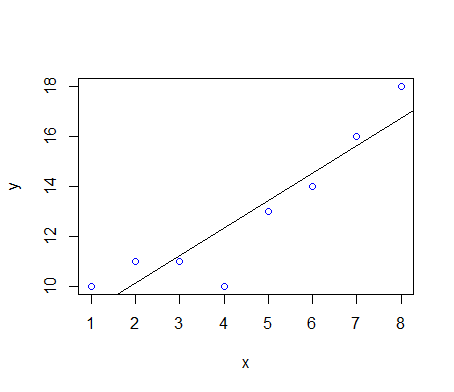
\includegraphics[scale=1]{LinReg.png}}
\question{}{$reg(0)=7.892857$\\
$reg(3.5)=11.767857$\\
$reg(5.75)=14.258929$}
\end{exercise}

\begin{exercise}[p=6]{}
\textbf{Classification:}\\
In Classification there are examples for each class given. Based on the parameters of these examples, new data is classified in the given classes.\\
For example given the personal data of a population, like salary, amount of children, position, etc. you can try to predict the education level. In this case education levels are the classes.\\\\
\textbf{Clustering:}\\
In Clustering the classes are unkonwn. Insted it tries to detect classes in given data by putting similar data points in the same class.\\
Clustering could be used in insurances to detect groups of customers who frequently report damages and so are costly for the company.\\\\
\textbf{Association:}\\
In Association the goal is to find related data points. Given the occurence of a specific data point the goal ist to give a probability for the occurence of other data points in the same data set.\\
For example you can predict that if somebody buys milk there is a 80\% chance the same person also buys cereal after analyzing shopping baskets of multiple customers.
\end{exercise}
\end{ukon-infie}
\end{document}